\scanpage{7}
\mspage{1}

% This entirely handwritten page has no handwriting envelope (briefv06).
% Main 01: certain accent, unresolved direction; two quotation ticks each side.
Soit \(M\) une catégorie (``\unsure{modèles|modéles}''). On suppose

% Main 02: accent direction remains uncertain; no point after monomorphique.
(i) Toute \unsure{flèche|fléche} de \(M\) est monomorphique

% Main 03: abbreviated old word, uncertain old stop, raised end without stop.
(ii) Tout \deleted{\unsure{autom|autom.}}\inserted{end} d'un élément de \(M\) est l'identité.

% Main 04: the reduced internal strokes do not resolve par.
Ex : \(M\) une catégorie définie \unsure{par} un ensemble ordonné

% Main 05: quotation ticks and a real blank, without a hyphen, in sous objets.
% Main 06: no point follows the terminal tilded D of the identification.
Pour tout \(D\in\mathrm{Ob}\,M\), soit \(\widetilde D\) l'ensemble (ordonné par ``inclusion'') des sous objets de \(D\). On identifie \(D\) au plus grand élément de \(\widetilde D\)

Soient \(D',D\in\mathrm{Ob}\,M\), alors l'application
% Main 07: a literal two-row map; M belongs under the final m of Hom.
% Lower u is indented; its barred shaft starts farther left and runs longer.
% The star is far left between row levels; the upper target has no comma.
\diagram{\begin{tikzcd}[ampersand replacement=\&,row sep=0pt,column sep=0pt]
{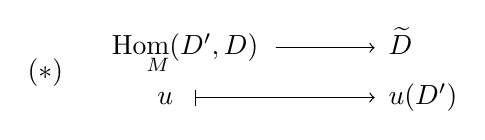
\begin{tikzpicture}[x=1em,y=1em,line width=.45pt,
 line cap=round,line join=round]
\node[anchor=base west,inner sep=0pt,outer sep=0pt] (homHo)
 at (0,0) {$\mathrm{Ho}$};
\node[anchor=base west,inner sep=0pt,outer sep=0pt] (homLast)
 at (homHo.base east) {$\mathrm m$};
\node[anchor=base west,inner sep=0pt,outer sep=0pt] (homArgs)
 at (homLast.base east) {$(D',D)$};
\node[anchor=north,inner sep=0pt,outer sep=0pt]
 at ([yshift=-.12em]homLast.south) {$\scriptstyle M$};
\node[anchor=base west,inner sep=0pt,outer sep=0pt]
 at (10,0) {$\widetilde D$};
\draw[->] ([xshift=.65em,yshift=.25em]homArgs.base east)--(9.5,.25);
\node[anchor=base west,inner sep=0pt,outer sep=0pt]
 at (1.65,-1.8) {$u$};
\draw[|->] (3,-1.55)--(9.5,-1.55);
\node[anchor=base west,inner sep=0pt,outer sep=0pt]
 at (10,-1.8) {$u(D')$};
\node[inner sep=0pt,outer sep=0pt] at (-2.4,-.65) {$(\ast)$};
\end{tikzpicture}}
\end{tikzcd}}
% Main 08: mixed first enclosure retained ahead of the two matched alternatives.
% Main 09: ens has no stop; the canceled de remains low-confidence;
% Phi is resolved, and inserted M- attaches before isomorphes.
est injective par \unsure{(i]|[i]|(i)}(ii), son image est formée de l'ens \deleted{\unsure{de}}
\(\Phi_{D'}(D)\subset\widetilde D\)
des sous-objets \(\Delta\) de \(D\) qui sont \inserted{\(M\)-}isomorphes à \(D'\).

\deleted{Soit \(K\) un ens. ordonné}

% Main 10--13 and 26: plain live N, deleted I, interlinear preordonne;
% the inserted sentence has only ordonne underlined; preceding M has its point.
Soit \(N\)\deleted{\(I\)} l'ens \inserted{préordonné} des classes d'isom. d'objets de \(M\). \inserted{Il est en fait \uline{ordonné}, grâce à (ii).}
% Main 14--18: unresolved forall/H, doubled N, canceled e/s, old D and live M;
% a raised star over n, and the first isom without a stop.
Pour \(\unsure{\forall|\mathrm H}\ n\in\mathbb N\), un\deleted{\unsure{e|s}} objet \(D_n\) de \deleted{\(D\)}\(M\) de classe \(\overset{\ast}{n}\) est déterminé à isom unique près,
% Main 19: reduced a/colon cluster plus a separate low down-right stroke.
% The literal stroke is neither a character candidate nor a therefore sign.
\begin{tikzpicture}[baseline=(causecluster.base),x=1em,y=1em,
 line width=.45pt,line cap=round]
\node[anchor=base west,inner sep=0pt,outer sep=0pt] (causecluster)
 at (0,0) {\unsure{à|:}};
\draw ([xshift=.12em,yshift=-.4em]causecluster.south east)
 --([xshift=.25em,yshift=-.62em]causecluster.south east);
\end{tikzpicture} cause de (ii),
% Main 20--22: ens without a stop; plain tilde D_n equals doubled J_n;
% resolved defini and the second isom without a stop.
donc l'ens ordonné \(\widetilde D_n=\mathbb J_n\) est défini à isom unique près.
% Main 23: dotted plui remains the first candidate; comma and old une are deleted.
On a donc \deleted{\unsure{plui|plus}, une}\inserted{une} famille
% Main 24: the family is a separate display.
\[
(\mathbb J_n)_{n\in\mathbb N}
\]
% Main 25: retain the observed footer wording and punctuation.
d'ens ordonnés, indexés par l'ensemble ordonné \(\mathbb N\).
% archive sheet number: 6
